\documentclass[12pt]{article}

\usepackage[utf8]{inputenc}
\usepackage[T1]{fontenc}
\usepackage[brazil]{babel}
\usepackage{graphicx}
\usepackage{geometry}
\usepackage{booktabs}
\usepackage{caption}
\usepackage{hyperref}
\geometry{margin=2.5cm}

\pagenumbering{gobble}

\begin{document}

\begin{titlepage}
    \begin{center}
        
        \vspace*{2cm}
        
        \begin{minipage}{0.4\textwidth}
            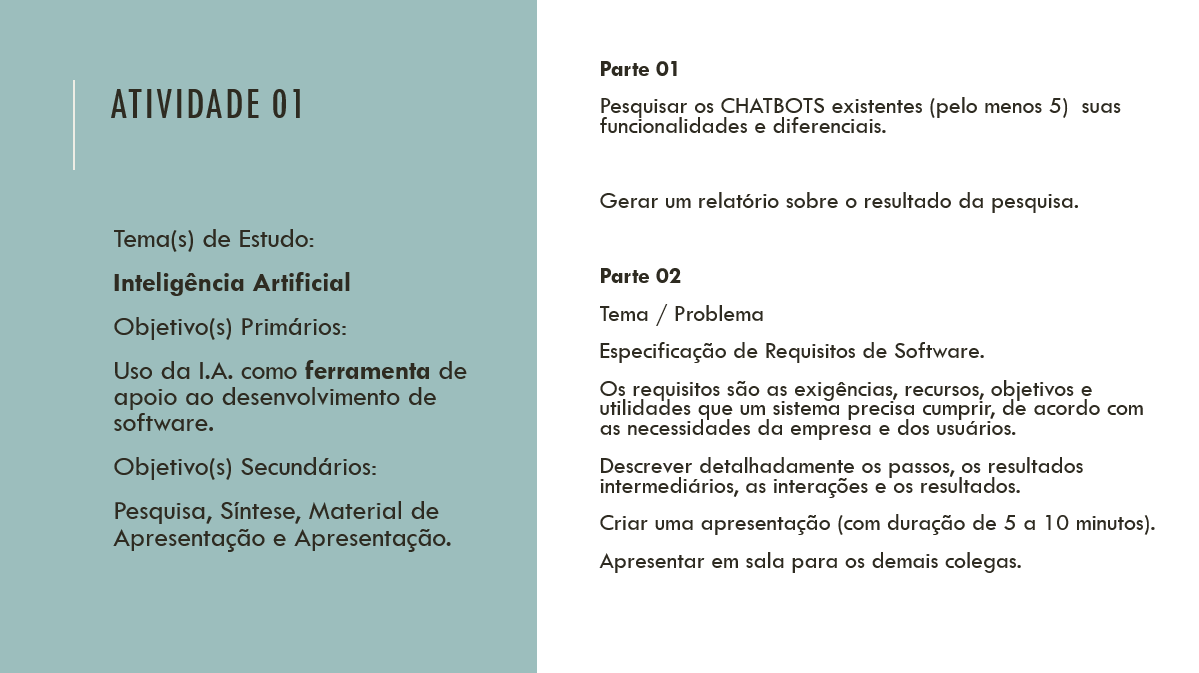
\includegraphics[width=\linewidth]{imagens/capa.png}
        \end{minipage}
        \hfill
        \begin{minipage}{0.5\textwidth}
            \raggedleft
            
            {\Huge \textbf{Inteligência Artificial}}\\[1.5cm]
            
            {\Large Otávio Augusto Brouwers Londero}\\[0.5cm]
            
            Ciência da Computação\\
            Turno: Noite\\
            Disciplina: Experiência Criativa: Explorando Computação e Inteligência Artificial\\

            \vfill
            
            Curitiba - PR\\
            2026
            
        \end{minipage}
        
    \end{center}
\end{titlepage}

\section{ChatBots:}
Aqui eu decidi escolher os ChatBots mais interessantes em minha opinião e "poderosos" do mercado por meio do site LiveBench e ARC Prize, e também falar de suas respectivas versões bases gratuitas.

\begin{itemize}
    \item \textbf{OpenAI (GPT-5.4 Thinking xHigh Effort)} - Modelo de ponta orientado a raciocínio e workflows agenticos. Indicado para pesquisa aprofundada, geração e revisão de código, automação de tarefas complexas e aplicações multimodais. O GPT-5.4 oferece suporte a janelas de contexto muito longas em variantes experimentais (configurações de 272k a ~1.05M tokens dependendo da variante) e apresenta modos ``Thinking'' focados em esforço de raciocínio. Versão base gratuita: o ChatGPT Free dá acesso restrito às variantes GPT-5 (variantes ``Instant''/padrão); o acesso ao GPT-5.4 Thinking completo costuma estar vinculado a planos pagos (Pro/Enterprise). 
    \item \textbf{Anthropic (Claude 4.6 Opus Thinking High Effort)} - Linha Opus (alta capacidade) e Sonnet (mid-tier) da Anthropic; Opus é otimizado para tarefas críticas (revisão de código, agentes confiáveis, produção empresarial) e tem suporte a janelas de contexto longas em modos beta. Sonnet funciona como alternativa com bom custo/benefício para POCs. Versão base gratuita: Sonnet costuma estar disponível em níveis gratuitos/pro com limites, enquanto Opus costuma requerer planos pagos ou acesso via API.
    \item \textbf{Google (Gemini 3.1 Pro Preview High*)} - Modelo Pro da família Gemini, projetado para eficiência de tokens, integração com ferramentas do ecossistema Google (Vertex AI, Search grounding) e capacidades multimodais. Indicado para pipelines de nuvem, agentes que usam ferramentas do Google e tarefas de engenharia. Versão base gratuita: acesso ao Gemini existe em ofertas consumidor (Bard / app) com recursos limitados; as variantes Pro/Preview são acessadas via Vertex/API (tiers pagas).
    \item \textbf{xAI (Grok 4)} - Grok 4 (e variantes \emph{Fast}) são modelos da xAI com foco em velocidade, custos reduzidos e janelas de contexto muito longas (variantes Fast anunciadas com janelas até milhões de tokens). Indicados para ingestão de grandes contextos, agentes em tempo real e aplicações que exigem baixa latência. Versões gratuitas: geralmente há camadas web/app com limites; variantes Fast são normalmente em planos pagos ou API.
    \item \textbf{Moonshot AI (Kimi K2.5 Thinking)} - Kimi (Moonshot) é um LLM com foco em raciocínio multimodal, integrações de busca/agent tools e paradigmas de \emph{visual coding}/agent-swarm. K2.5 é uma versão otimizada para eficiência em tasks multi-step. Versão base gratuita: a plataforma Kimi disponibiliza acesso via app/web com camadas gratuitas e limites em volume/performance.
\end{itemize}

\subsection*{Versões base gratuitas (observações rápidas)}
\begin{itemize}
    \item OpenAI: ChatGPT Free normalmente fornece acesso às variantes padrão/Instant da família GPT-5; acesso ao GPT-5.4 Thinking completo está atrelado a planos pagos.
    \item Anthropic: Sonnet costuma ser o modelo default para planos Free/Pro; Opus (4.6) é premium.
    \item Google: versões consumidoras do Gemini (Bard, app) existem com limites; acessos Pro/Preview via Vertex AI são pagos.
    \item xAI: Grok tem experiências web gratuitas com limites; variantes Fast/enterprise são pagas via API.
    \item Moonshot: Kimi oferece camadas gratuitas no app; acesso de alto volume/baixa latência normalmente pago.
\end{itemize}
\end{document}